\section{Realizzazione}

Per la realizzazione di questo sito web abbiamo deciso di renderizzare tutti gli
elementi lato server, utilizzando PHP per la gestione delle richieste e delle
risposte. In particolare, la cartella \texttt{src} contiene tutti i file che
riguardano il back-end e la struttura gerarchica data dalle cartelle riflette la
divisione in moduli del codice.\\
Dunque ci sono i seguenti moduli:
\begin{itemize}
	\item \textbf{template}: contiene tutti i file html che sono utilizzati per
	      la creazione delle pagine web;

	\item \textbf{page}: contiene le classi php che si occupano di creare una
	      pagina web per interno oppure solo una porzione di essa;

	\item \textbf{model}: contiene le classi php che si occupano di gestire i
	      dati, le operazioni sul database o la logica di business, come ad
	      esempio la gestione delle sessioni, ovvero dei cookie;

	\item \textbf{controller}: contiene le classi php che si occupano di
	      gestire le richieste e le risposte, assemblano i servizi e le pagine
	      per fornire una risposta coerente all'utente;

	\item \textbf{test}: finalmente, test contiene i file php che si occupano di
	      testare le classi php del progetto. Approfondiamo questo modulo nella
	      sezione \ref{sec:test}.
\end{itemize}

\subsection{Page}

In questo modulo viene definita la classe \texttt{Page} che viene così definita:

\begin{lstlisting}[language=PHP]
class Page
{
    protected function getContent($path);
    protected function setTitle($title);
    protected function addKeywords($keywords);
    protected function setNav($nav);
    protected function setBreadcrumb($breadcrumb);
    protected function takeOffCircularReference($content);
    public function setPath($path);
    public function render();
    public function error($message);
}
\end{lstlisting}

Vogliamo portare l'attenzione su alcuni metodi:
\begin{itemize}
	\item \texttt{takeOffCircularReference}: questo metodo si occupa di
	      rimuovere i link circolari presenti nel contenuto della pagina;

	\item \texttt{render}: questo metodo viene sovrascritto dalle classi figlie,
	      di modo da uniformare la creazione di una pagina web, senza dover
	      modificare il layout di base delle pagine.
\end{itemize}

\subsection{Model}

Il model interagisce con il database, per cui la struttura delle classi
rispecchia quella del database, quindi riportiamo solo la struttura del
database, che si evince dal diagramma in figura \ref{fig:Database} e riportiamo
una classe di esempio per mostrare come vengono gestiti i dati.

\begin{figure}[h]
	\centering
	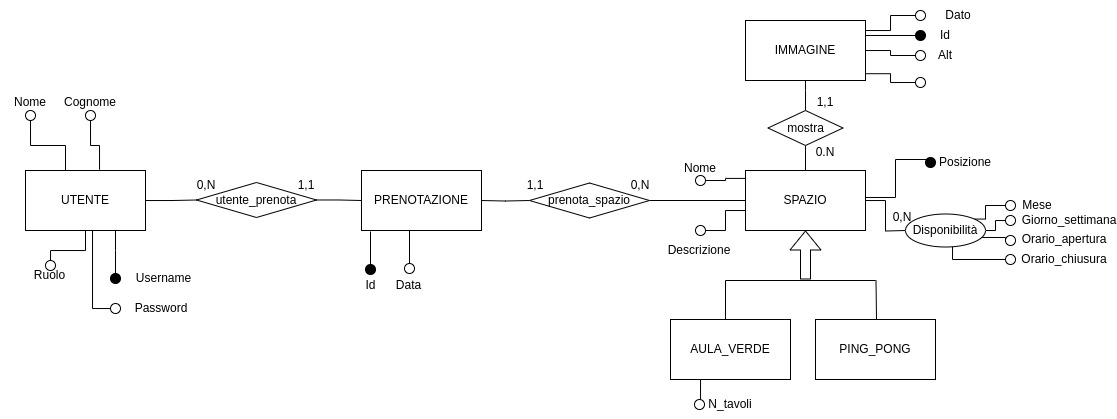
\includegraphics[width=0.9\textwidth]{figures/Database}
	\caption{Diagramma del database.}
	\label{fig:Database}
\end{figure}

Per stabilire la connessione con il database viene utilizzata l'estensione
\texttt{MySQLi} di PHP.\\
Abbiamo deciso di utilizzare la classe \texttt{Utente} come esempio. Notiamo che
viene utilizzata la classe \texttt{Database} per stabilire una connessione con
il database e per assicurarci che la connessione sia unica: infatti questa
classe implementa il pattern \texttt{Singleton}. La classe \texttt{Model} ha un
istanza della classe \texttt{Database} e la utilizza per eseguire le query; la
classe \texttt{Model} definisce i metodi per interagire con il database.
Finalmente, la classe \texttt{Utente} estende la classe \texttt{Model} e
implementa le operazioni CRUD sull'entità \texttt{Utente}.
Infine, notiamo che la classe \texttt{Utente}, quando inserisce un nuovo utente
all'interno del database utilizza la funzione \texttt{password\_hash} della
libreria standard di PHP per criptare la password, in modo tale che essa non sia
salvata in chiaro nel database e che un eventuale attacco non possa recuperare
la password degli utenti.

\begin{figure}[h]
	\centering
	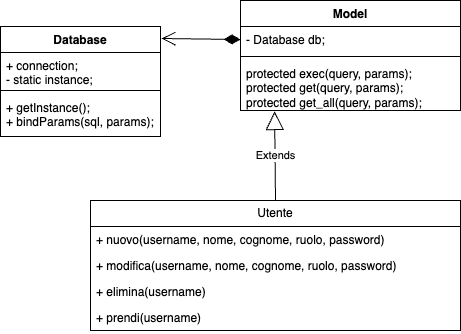
\includegraphics[width=0.5\textwidth]{figures/model}
	\caption{Diagramma delle classi del model}
	\label{fig:model}
\end{figure}

\subsection{Controller}

Finalmente abbiamo implementato il controller, che si occupa di utilizzare i due
moduli spiegati in questa sezione per gestire le richieste dell'utente. In
particolare, una richiesta ad un controller ritorna una pagina web, che viene
creata utilizzando il modulo \texttt{page}. In figura \ref{fig:controller} è
riportato il diagramma delle classi del controller. Notiamo che viene definta
una classe \texttt{Router} che gestisce un array di \texttt{Endpoint}. Un router
si occupa di individuare e delegare ciascuna richiesta che riceve ad uno dei
suoi endpoint. Un endpoint estende la classe \texttt{Endpoint} e implementa il
metodo \texttt{handle}, che si occupa di gestire la richiesta.
\begin{figure}[h]
	\centering
	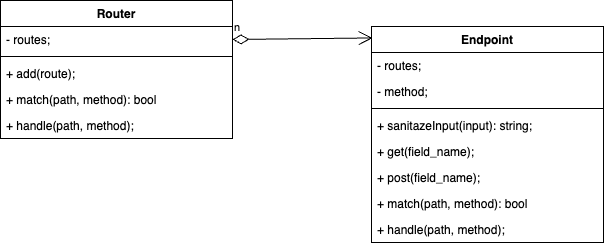
\includegraphics[width=0.5\textwidth]{figures/controller}
	\caption{Diagramma delle classi del controller.}
	\label{fig:controller}
\end{figure}
